\documentclass[12pt,fleqn]{article}\usepackage{../common}
\begin{document}


$$ 
c = \frac{ 2c_m}{1 + \cosh |b_c(t-t_{mc})|   }
$$


\begin{minted}[fontsize=\footnotesize]{python}
from scipy.optimize import fmin
import pandas as pd
from numpy.linalg import *
df = pd.read_csv('oil1.csv',sep='\s*')

def hubbard(w):
    yfit = (2*w[0]) / (1+cosh( w[1] * (df['year']-w[2])))
    diff = df['oil'] - yfit
    e=norm(diff)
    return e

v = fmin(hubbard, [2, 2, 1990], maxiter=100000, maxfun=10000)
print v
\end{minted}

\begin{verbatim}
Optimization terminated successfully.
         Current function value: 52.188303
         Iterations: 193
         Function evaluations: 352
[  8.38712818e+01  -4.77382424e-02   2.00814756e+03]
\end{verbatim}

\begin{minted}[fontsize=\footnotesize]{python}
df = df.set_index('year')
df['oil'].plot(oil)
plt.savefig('peak_01.png')
\end{minted}

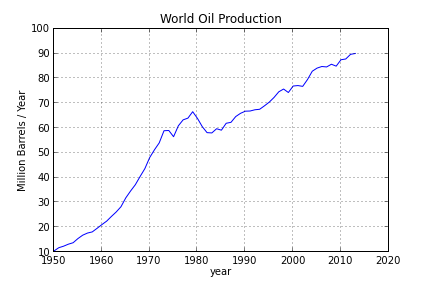
\includegraphics[height=6cm]{peak_01.png}

\url{http://www.earth-policy.org/Updates/2007/Update67_data2.htm#table1}

\url{http://en.wikipedia.org/wiki/Hubbert_curve}

\url{http://www.eia.gov/cfapps/ipdbproject/iedindex3.cfm?tid=5&pid=53&aid=1&cid=ww,&syid=1980&eyid=2013&unit=TBPD}

\url{http://www.countercurrents.org/mushalik270314.htm}


\end{document}
